En esta sección se describen las funciones y configuración establecida de los componentes de VCF, tanto los desplegados con la herramienta VLC como los instalados manualmente para completar las funcionalidades de la solución.

\begin{subsubsection}{Diseño de VMware vCenter Server}
  \label{subsubsec:diseno-vcenter}
El componente VMware vCenter Server es el punto de acceso y de control de todas las VMs localizadas en los hosts ESXi bajo su dominio. Esta instancia de vCenter Server contiene un dominio con un cluster vSphere que agrupa a los cuatro hosts ESXi que forman el Magement Domain. Estos hosts se denominan respectivamente \textit{esxi-1}, \textit{esxi-2}, \textit{esxi-3} y \textit{esxi-4}, el primero cuenta con 96 GB de memoria RAM, el resto con 64 GB de memoria RAM y cada host tiene un total de 19,9 GHz de CPU. Desde VMware vCenter Server el administrador del SDDC gestiona los recursos de las VMs de cada componente, monitoriza los recursos del entorno, administra la creación y asignación de roles, permisos y usuarios, gestiona los grupos de discos que forman el datastore de VMware vSAN, determina las redes a las que se conecta cada componente, establece la configuración de disponibilidad y recuperación ante fallos proporcionada por VMware vSphere, en definitiva, VMware vCenter Server es el punto desde donde se controla y administra la infraestructura.
\begin{figure}[h]
  \centering
  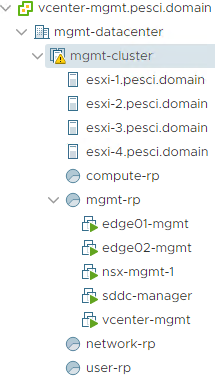
\includegraphics[width=0.2\textwidth]{imaxes/pruebaconcepto/clusterVCenterServer.png}
  \caption{Dominio de la instancia de VMware vCenter Server.}
  \label{fig:cluster-vCenter-Server}
\end{figure}
\FloatBarrier
En la imagen anterior se muestra el dominio \textit{vcenter-mgmt.pesci.domain} de la instancia de VMware vCenter Server y el cluster vSphere \textit{mgmt-cluster} donde se alojan los componentes del Management Domain. 
% Este cluster incluye cuatro \textit{resource pools}, uno de ellos (\textit{mgmt-rp}) contiene las VMs de los componentes dedicados al Management Domain.
%  Con vCenter Server se simplifica la escalabilidad del SDDC, la gestión de actualizaciones para los componentes es más sencilla, permite determinar roles específicos y responsabilidades y permite aislar las redes de otras instancias de vCenter Server. Además, para gestionar vSpehere SSO Domain, VMware vCenter Server contiene embebido el componente PSC con todos los servicios necesarios. 
%  En caso de que existan varios \textit{Workload Domain} se puede habilitar el modo \textit{Enhanced Linked Mode} para poder gestionar todas las instancias de vCenter Server de forma centralizada desde un único vSphere Client.
% Por lo anterior, en el \textit{management domain} se despliega una instancia de VMware vCenter Server que incluye un cluster de VMware vSphere.

\end{subsubsection}

\begin{subsubsection}{Diseño cluster VMware vSphere}
\label{subsubsec:diseno-vsphere}
Los cuatro hosts desplegados para el Management Domain están agrupados en un cluster de VMware vSphere, donde se encuentran las VMs de los componentes de VCF (figura \ref{fig:cluster-vCenter-Server}). Gracias a dos funcionalidades de este componente, se establece una configuración para mantener activas las VMs desplegadas dentro de este cluster mediante el balanceo de forma automatizada del consumo de recursos y la recuperación del servicio de las VMs cuando alguna sufre un fallo. Estas funciones de VMware vSphere son:
\begin{itemize}
  \item vSphere High Availability: establece una cantidad de recursos que se reserva de los disponibles en el cluster vSphere, y se encarga de reiniciar una VM cuando deja de estar operativa. Para este cluster se establece una reserva el 25\% de la CPU total y el 25\% de la memoria RAM total. De esta forma, se asegura que una cuarta parte de los recursos disponibles están reservados para reiniciar, en un host diferente, una VM que ha dejado de funcionar.
  
  \item vSphere DRS: se encarga de migrar VMs de un host a otro dentro del cluster vSphere,con el objetivo de balancear la carga de trabajo entre los hosts disponibles. Usando este servicio se garantiza que cada VM obtiene la capacidad necesaria para funcionar correctamente, y aumenta la eficiencia del cluster al hacerse un mejor uso de sus recursos. Para realizar las migraciones entre hosts, vSphere DRS utiliza la funcionalidad vMotion, el cual permite mover una VM de un host a otro manteniendo el estado en el que se encontraba, y manteniendo activo el servicio de la VM. Por ejemplo, si el consumo de recursos de un host está alrededor del 100\%, vSphere DRS lo detecta e inicia la migración de la VM mediante vMotion, a otro host con recursos disponibles. 
\end{itemize}

Combinando estas dos funcionalidades, las tareas de mantenimiento se reducen ya que es VMware vSphere quien, de forma automática y transparente se encarga de monitorizar el estado de las VMs y los hosts, de optimizar el uso de recursos y de asegurarse de que existen suficientes recursos para la ejecución de todos los flujos de trabajo.

% Dentro de un \textit{workload domain} pueden existir varios clusters vSphere con diferentes características según su finalidad. Los hosts ESXi que lo forman pueden ser de diferentes tamaños teniendo en cuenta que se pueden usar menos hosts ESXi de mayor capacidad o más hosts con menores prestaciones, el coste de cada host ESXi, el uso que se le va a dar al cluster y las características máximas y mínimas del cluster vSphere. Debido a la limitada cantidad de recursos que ofrece el host físico donde se realiza el despliegue, para el \textit{management domain} se utiliza un único cluster vSphere con de 4 hosts de los cuales se reserva un host para proveer redundancia. Todos los hosts ESXi cuenta con 64GB de memoria RAM menos uno que tiene 32 GB, y 19.9GHz de CPU. Dentro del cluster hay que configurar los servicios vSphere HA y vSphere DRS para proteger los componentes del SDDC. La configuración que se establece en el \textit{management domain} es la siguiente:
% En caso de que el \textit{management domain} esté extendido en dos AZ entonces se requieren 4 hosts en cada AZ para proporcionar redundancia y disponibilidad en caso de caída de una de las AZ.

% \begin{itemize}
%     \item \textbf{vSphere High Availability}: en este servicio la propiedad \textit{Admission Control Policy} permite establecer la cantidad de recursos reservados en caso de fallo y como se establece el cálculo de esos recursos. En el \textit{management domain} se configura para el fallo de al menos un host y reserva de recursos según un porcentaje, reservando así el 25\% de la CPU y el 30\% de la memoria RAM ya que funciona mejor cuando las VM usan mucha CPU y memoria. La otra propiedad que se debe habilitar para el correcto funcionamiento del servicio es \textit{VM and Application Monitoring}, que se encarga de reiniciar las VM en caso de caída.
    % que puede ser según el número hosts que pueden fallar en el cluster, según un porcentaje de reserva de rescursos o especificando el host donde se recolocan las VM del host caído.  RAM.  
%     \item \textbf{vSphere DRS}: 
% este servicio permite migrar VMs de un host ESXi a otro dentro del mismo cluster vSphere para equilibrar la carga de trabajo y mantener las VMs activas en caso de caída de alguno de los hosts. Se activa usando la opción por defecto \textit{Fully Automated} ya que aporta el mejor balance entre consumo de recursos y migraciones de VM innecesarias. Adicionalmente también se pueden establecer reglas para determinar el orden de encendido de las VMs pertenecientes a un mismo grupo. 
%     %En caso de que exista más de una AZ, se deben crear grupos de VM y de hosts de cada AZ para luego implementar reglas de afinidad para que las VM de una AZ no sean migradas a otra AZ ya que esto puede afectar al rendimiento de la VM. 
% \end{itemize}
% En el modelo consolidado se debe crear un único cluster con un mínimo de cuatro hosts ESXi ya que uno de los hosts se utiliza para asegurar la disponibilidad del almacenamiento vSAN cuando hay algún host inactivo. Este modelo proporciona capacidad de un único fallo por cluster.
\end{subsubsection}

\begin{subsubsection}{Diseño de red para el cluster vSphere}
  A parte de controlar la disponibilidad de los recursos, VMware vSphere también se encarga de gestionar las redes a las que se conecta cada VM, permitiendo separar cada tipo de tráfico en subredes y asignarles unas propiedades específicas. Para llevar esto a cabo y que las VMs puedan conectarse a la red externa y comunicarse con el resto de VMs, dentro del cluster vSphere se crea un vShpere Distributed Switch (vDS), en el cual se configuran puertos a los que se conectan las VMs alojadas en el cluster vSphere.
  % que las VMs tengan conectividad con la red externa y con el resto de VMs, en el cluster vSphere, se crea un vShpere Distributed Switch (vDS), en el cual se configuran puertos a los que se conectan las VMs alojadas en el cluster vSphere.
  \begin{figure}[h]
    \centering
    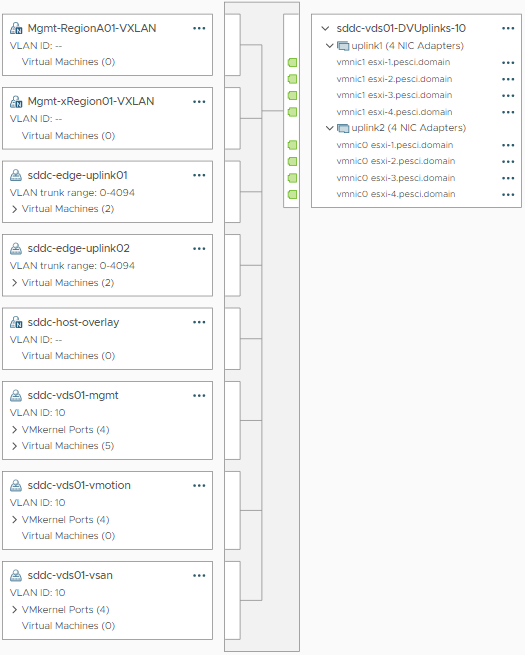
\includegraphics[width=0.5\textwidth]{imaxes/pruebaconcepto/distributedSwitchEntornoFinal.png}
    \caption{Contenido de vSphere Distributed Switch \textit{sddc-vds01}.}
    \label{fig:port-groups-vSwitch-vSphere}
  \end{figure}
  \FloatBarrier
  Como se muestra en la figura anterior, el vDS creado para el cluster vSphere del Management Domain contiene varios puertos, donde hay VMs conectadas, y dos interfaces uplink (\textit{sddc-vds01-DVUplinks-10}). Estas dos interfaces, \textit{uplink1} y \textit{uplink2}, representan las interfaces de red físicas de cada host y son las que dan salida al tráfico de las VMs hacia la red física del entorno. Cada uno de los puertos tiene una función específica, estos son, \textit{sddc-vds01-mgmt}, dedicado al tráfico de configuración y gestión que los componentes de VCF envían entre sí, \textit{sddc-vds01-vmotion}, dedicado al tráfico de las migraciones de VMs entre hosts llevadas a cabo por la funcionalidad vMotion, \textit{sddc-vds01-vsan}, usado por las VMs para acceder al datastore de VMware vSAN, \textit{sddc-edge-uplink01} y \textit{sddc-edge-uplink02}, puertos usados por los componentes de VMware NSX-T para dar salida, hacia la red física, al tráfico de las redes virtuales que gestiona este componente de VCF. Los demás puertos que se muestran en la imagen son generados de forma automática por VMware NSX-T. 
  En la configuración de cada puerto, se establece la VLAN que se asigna a su tráfico, las interfaces uplink por las que se transmite su tráfico hacia la red física, cómo se balancea la carga entre cada interfaz uplink, y la prioridad que se asigna a su tráfico respecto al resto de puertos. Los puertos, cuyo tráfico tiene mayor prioridad son \textit{sddc-vds01-vsan} y \textit{sddc-vds01-vmotion}, con el fin de asegurarse de que obtienen el suficiente ancho de banda y así facilitar la transmisión de archivos de gran tamaño. 
  % re cada puerto se establecen varias propiedades En cuanto a las propiedades del tráfico, dentro del vDS se determina qué tráfico tiene más prioridad sobre los recursos de red, en este caso se establece el tráfico de los puertos \textit{sddc-vds01-vsan} y \textit{sddc-vds01-vmotion} como los de mayor prioridad, para asegurarse de que obtienen el suficiente ancho de banda y así facilitar la transmisión de archivos de gran tamaño. También, para cada puerto, se establece la VLAN con la que se etiqueta el tráfico, qué interfaces de red físicas se deben utilizar y como debe balancear el tráfico entre estas.
\\
  De esta forma, las propiedades del tráfico de cada subred son configuradas a través de VMware vSphere. Esto simplifica el proceso administración y configuración de las subredes del entorno, ya que una vez configurados los dispositivos de red físicos, el router VyOS en este caso, con las direcciones IP, las etiquetas VLAN y MTU correspondientes, la monitorización de la red y la configuración de la calidad del servicio se realizan desde VMware vSphere.
\end{subsubsection}

\begin{subsubsection}{Diseño almacenamiento VMware vSAN}
  \label{subsubsec:diseno-vsan}
  Los hosts del Management Domain utilizan como almacenamiento un datastore del componente VMware vSAN. Está formado por 16 discos SDD agrupados en cuatro grupos con configuración All-Flash, cada grupo está asociado a un host. Para mantener la disponibilidad de los ficheros almacenados en el datastore, se establece la opción \textit{Failures-To-Tolerate} (FTT) igual a uno. De esta forma, VMware vSAN mantiene dos copias de los archivos generados por las VMs y las coloca en grupos de discos distintos, de forma que si ocurre un fallo en alguno de los hosts las VM seguirán teniendo acceso a sus archivos. Esta configuración equivale a tener un sistema de almacenamiento RAID 1, pero con la ventaja de que no se ha modificado la configuración del hardware y, si fuera necesario, se podría aumentar el número de réplicas simplemente editando el valor de FTT desde el portal de VMware vCenter Server. Como se muestra en la siguiente figura, VMware vSAN mantiene una copia del mismo archivo en dos hosts/grupos de discos diferentes, mientras la configuración física de cada grupo de discos es de tipo RAID 0. Las máquinas virtuales acceden al \textit{datastore} a través de una subred que utiliza su propia VLAN y a la que todos los hosts están conectados.
  \begin{figure}[h]
    \centering
    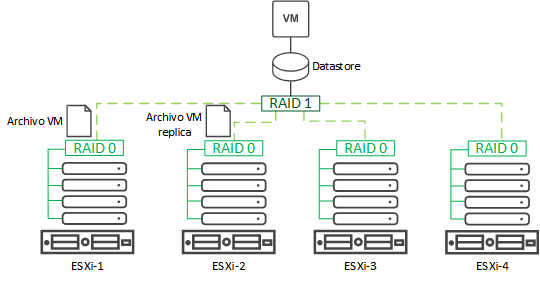
\includegraphics[width=0.8\textwidth]{imaxes/pruebaconcepto/vSANconfig.png}
    \caption{Ejemplo de como se almacena un archivo con VMware vSAN y FTT igual a uno}
    \label{fig:vSAN-config-FTT}
  \end{figure}
  \FloatBarrier
  Utilizar el sistema de almacenamiento de VMware vSAN supone una gran mejora respecto al sistema de almacenamiento basado en LUNs, utilizado actualmente en el CPD del CITIC. VMware vSAN monitoriza los dispositivos de almacenamiento y configura la redundancia de los archivos de forma dinámica y sencilla, permitiendo establecer una configuración específica según sea necesario, sin modificar los dispositivos físicos de almacenamiento. Con el sistema basado en LUNs es obligatorio modificar la estructura y configuración de los dispositivos físicos cada vez que se quiera establecer una configuración de redundancia diferente en el sistema de almacenamiento, lo cual supone un gran coste para el administrador y un aumento de los riesgos. Si tomamos el ejemplo de la figura anterior, la redundancia el sistema gestionado por VMware vSAN, con FTT igual a 1, podría ser aumentada estableciendo la opción de configuración FTT igual a 2. Así, se crearía una nueva copia del archivo en un tercer host/grupo de discos mientras la configuración física se mantiene igual.
  % sts participantes, soporta el fallo de un host lo cual permite dejar hosts fuera de servicio para tareas de mantenimiento. Esto es posible gracias a que con FTT (\textit{Failures-To-Tolerate}) igual a 1 se mantiene la redundancia de los datos almacenados en el \textit{datasotore}, en uno de los hosts. Cada grupo de discos cuenta con cuatro discos uno de ellos para caché, 16 discos en total. Para hacer disponible este servicio de almacenamiento, todos los hosts deben estar conectados a la subred generada para VMware vSAN y utilizar una VLAN para separar su tráfico.

\end{subsubsection}

% Si bien en VMware Cloud Foundation existe VMware NSX-T, un componente dedicado únicamente a la administración de la red del SDDC, es desde VMware vSphere dónde se encuentran los elementos para establecer redes que separen cada tipo de tráfico de los componentes del SDDC. Estas redes se configuran en base a los siguientes aspectos:
% \begin{itemize}
%     \item Separar el tráfico de cada servicio para mejorar la eficiencia de la red y la seguridad. Así se puede ajustar las características de cada red, como el ancho de banda o la latencia, a las necesidades de cada servicio.
%     \item Utilizar un único vSphere Distributed Switch por cluster donde se añade un \textit{port group} por cada servicio.
%     % \item Mejorar el rendimiento usando NICs de tipo VMXNET3 en las máquinas virtuales.
%     \item Las NICs físicas de cada host ESXi conectados a un mismo vSphere Distributed Switch están conectadas también a la misma red física.
%     % \item Aquellas redes que se dedican a servicios de la infraestructura deben estar configuradas con puertos tipo \textit{vmkernel}.
% \end{itemize}
% Para el \textit{management domain} del SDDC se crea un único vSphere Distributed Switch llamado \textit{sddc-vds01} con la siguiente configuración:
% \begin{itemize}
    
%     \item Se establece un MTU igual 9000 Bytes para permitir el tráfico de \textit{jumbo frames} ya que son requeridos por algunos de los servicios.
    
%     \item Se habilita el servicio \textit{Network I/O} que permite establecer un nivel de prioridad a cada tipo de tráfico. Esto se realiza estableciendo limites de ancho de banda, políticas de balanceo de carga y reserva de recursos para un tipo de tráfico asociado a un servicio. Por cada tipo de tráfico hay cuatro aspectos que se pueden configurar que son \textit{Shares} (indica el \% de ancho de banda que se le da a un tipo de tráfico, el tipo de tráfico que tenga un mayor valor en \textit{Shares} tendrá más prioridad a la hora de usar los recursos), \textit{Reservation} (indica el valor de ancho de banda que se reserva para el tipo de tráfico) y \textit{Limit} (establece un valor máximo para el ancho de banda de un tipo de tráfico). En el \textit{management domain} los tipos de tráfico más relevantes que se deben configurar son los siguientes:
%     \begin{itemize}
%       \item \textit{Management Traffic}: el valor \textit{Shares} se establece al 50\% (\textit{Normal}) lo cual le da mayor prioridad que el resto de tipos. El resto de valores no se modifican.
%       \item \textit{vSphere vMotion Traffic}: el valor \textit{Shares} se establece al 25\% (\textit{Low}) ya que durante el estado normal del entorno este tipo de tráfico no es muy importante. El resto de valores no se modifican.
%       \item \textit{vSAN Traffic}: el valor \textit{Shares} se establece al 100\% (\textit{High}) para garantizar que este servicio recibe la cantidad de ancho de banda que necesita. El resto de valores no se modifican.
%       \item \textit{Virtual Machine Traffic}: el valor \textit{Shares} se establece al 100\% (\textit{High}) para garantizar que las VMs siempre tienen acceso a la red ya que son una parte importante del SDDC. El resto de valores no se modifican.
%     \end{itemize}
    
%     \item Para detectar errores de compatibilidad entre la configuración del vSphere Distributed Switch y la red física se habilita el servicio \textit{Health Check}. Este se encarga de comprobar si la configuración de cada VLAN y MTU se adapta a la configuración de la capa física.
    
%     \item Como puertos de salida \textit{Uplink} se configuran las interfaces físicas \textit{vmnic0} y \textit{vmnic1}. Como vDS es un componente distribuído, en cada host se usarán ambas interfaces de red como \textit{uplinks}.
    
% \end{itemize}
% En este vSpehere Distributed Switch para el Management Domain se configuran los siguientes \textit{port groups}, que son de tipo \textit{Distributed port group} y de tipo \textit{Uplink port group}. Además, el vDS está configurado sobre los cuatro hosts por lo tanto todos tienen acceso a todos los \textit{port groups}:
% \begin{itemize}
       
%         \item \textbf{Management port group}: es un \textit{Distributed port group} que comunica a todos los hosts ESXi entre si y transmite el tráfico entre los diferentes componentes de VMware Cloud Foundation, es decir, por este \textit{port group} circulan los comandos de configuración y gestión que los componentes del SDDC se envían entre ellos. Tiene el nombre \textit{sddc-vds01-mgmt}, a él se conectan las VMs \textit{vcenter-mgmt}, \textit{sddc-manager}, \textit{nsx-mgmt-1},\textit{edge01-mgmt} y \textit{edge02-mgmt}. Utiliza la subred con IP 10.0.0.0, máscara de red 255.255.255.0, VLAN 10 y MTU igual a 1500 Bytes. Esta red debe ser configurada también en la infraestructura física.
        
%         \item \textbf{vMotion port group}: es un \textit{Distributed port group} que está dedicado al tráfico del componente vSphere vMotion para realizar las migraciones de máquinas virtuales de un host a otro. Tiene el nombre \textit{sddc-vds01-vmotion} y utiliza la subred con IP 10.0.4.0, máscara de red 255.255.255.0, VLAN 10 y MTU igual a 8940 Bytes.
        
%         \item \textbf{vSAN port group}: es un \textit{Distributed port group} que está dedicado al servicio de almacenamiento VMware vSAN y por él los hosts acceden al almacenamiento del SDDC. Tiene el nombre \textit{sddc-vds01-vsan} y utiliza la subred con IP 10.0.8.0, máscara de red 255.255.255.0, VLAN 10 y MTU igual a 8940 Bytes.
        
%         \item \textbf{Edge Uplink port group}: es un \textit{Distributed port group} dedicado a las conexiones del component NSX-T Edge que se dedica a dar acceso a determinados servicios y para proporcionar a otros \textit{workload domain} conexión con la red externa. Están gestionados por VMware NSX-T ya que dan servicio a sus componentes. En el entorno existen dos \textit{port groups} para proporcionar redundancia y alta dispobilidad, uno llamado \textit{sddc-edge-uplink01} cuyas instancias están configuradas bajo la red con IP 172.27.11.0 y con máscara de red 255.255.255.0, y otro llamado \textit{sddc-edge-uplink02} cuyas instancias están configuradas bajo la red con IP 172.27.12.0 y máscara de red 255.255.255.0. Ambos \textit{port groups} están configurados como VLAN Trunk (por ellos puede circular tráfico de cualquier VLAN) y tienen un MTU de 8940 Bytes. En ambos hay configuradas las dos VMs llamadas \textit{edge01-mgmt} y \textit{edge02-mgmt}. Estas dos redes también se deben configurar en la infraestructura física.
        
%         \item \textbf{Uplink port group}: se trata de un \textit{Uplink port group} al que se le asignan las NICs físicas de cada host para establecer políticas sobre el tráfico que se dirige desde los hosts y VMs hacia fuera del vSphere Distributed Switch. Con el nombre \textit{sddc-vds01-DVUplinks-10}, en él están configuradas las dos NICs físicas de cada host, cada una en una interfaz \textit{uplink}.
        
% \end{itemize}
% \begin{figure}[h]
%   \centering
%   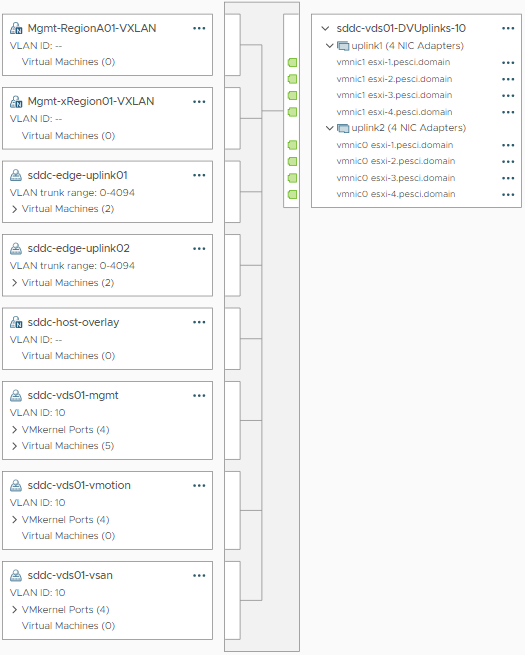
\includegraphics[width=0.4\textwidth]{imaxes/pruebaconcepto/distributedSwitchEntornoFinal.png}
%   \caption{Contenido de vSphere Distributed Switch \textit{sddc-vds01}.}
%   \label{fig:port-groups-vSwitch-vSphere}
% \end{figure}
% \FloatBarrier
% En la imagen anterior se muestran todos los \textit{Distributed Port Groups} y \textit{Uplink port group} que se alojan en el vSphere Distributed Switch (\textit{sddc-vds01}) dedicado al \textit{management domain}. En el \textit{port group} \textit{sddc-vds01-DVUplinks-10} se muestra como cada interfaz \textit{uplink} se mapea con una interfaz física (vmnic) de cada host ESXi. Los \textit{port groups} \textit{mgmt-Region01A-VXLAN}, \textit{mgmt-xRegion01-VXLAN} y \textit{sddc-host-overlay} son generados y administrados por el componente VMware NSX-T como se explicará más adelante. Cada \textit{port group} informa de cuantas VMs y hosts ESXi tiene conectados.

% La configuración que se aplica a cada \textit{Distributed port group} descrito anteriormente es la siguiente:
% \begin{itemize}
%   \item \textit{Port binding}: permite indidcar como se gestionan los puertos de un \textit{port group} cuando se añade o elimina una VM. Tiene dos opciones de configuración, la primera se denomina \textit{Static Port Binding} y su función consiste en asignar un puerto dentro del \textit{port group} a la VM que se conecta y solo se elimina cuando la VM es borrada. La segunda opción se denomina \textit{Ephemeral Port Binding} y consiste en que el puerto se asigna a la VM cuando esta se enciende y se elimina cuando se apaga o elimina. Para los \textit{port groups} \textit{sddc-vds01-vsan} y \textit{sddc-vds01-vmotion} se configura la opción \textit{Static Port Binding} ya que así se asegura que las VMs se conectan siempre al mismo puerto lo cual permite mantener datos históricos y hacer monitoreo a nivel de puerto. Para los \textit{port group} \textit{sddc-vds01-mgmt}, \textit{sddc-edge-uplink01} y \textit{sddc-edge-uplink02} se configura la opción \textit{Ephemeral Port Binding} ya que, como el tráfico que circula por ellos es el que gestiona todos los componentes del SDDC y dan acceso a otras redes externas, se elimina la dependencia con el estado de VMware vCenter Server permitiendo que la comunicación continúe aunque VMware vCenter Server no se encuentre operativo.

%   \item \textit{Load Balancing}: indica como se distribuye el tráfico de salida de cada VM/host que se encuentran en el \textit{port group} entre las NICs físicas. Se selecciona \textit{Route based on physical NIC load}, es decir, el tráfico de una VM se transmite por una única NIC por lo que si esa NIC física está saturada, se asignará otra NIC física a la VM.
  
%   \item \textit{Network failure detection}: esta opción permite establecer como debe determinar el \textit{port group} que alguna de las NICs físicas está fuera de servicio. Se selecciona \textit{Link status only} para que esto se determine según el estado que le transmite la NIC física, así se pueden detectar los fallos que ocurren en la red física.
  
%   \item \textit{Notify switches}: se habilita para permitir a los host enviar \textit{frames} a los switches físicos para que estos conozcan la localización de las VM que están funcionando en cada host.
  
%   \item \textit{Failback}: permite determinar como se reactiva una NIC cuando esta se recupera de un fallo. Se habilita para establecer que la NIC se marcará como activa inmediatamente después de que se haya recuperado. Esta opción se debería desactivar en caso de que el estado de la NIC sea inestable.
  
%   \item \textit{Failover Order}: permite determinar que uplinks se deben utilizar, los que se seleccionan como \textit{active} son los que se utilizarán por defecto, los que se seleccionan como \textit{stand by} se usarán cuando los uplinks marcados como \textit{active} se encuentren desactivados. Se seleccionan las dos interfaces \textit{uplink} disponibles en el estado \textit{active}. Para el \textit{port group} \textit{sddc-edge-uplink01} se selecciona la interfaz \textit{uplink1} como activa y se deja sin usar la interfaz \textit{uplink2}, mientras que se configura de forma contraria en el \textit{port group} \textit{sddc-edge-uplink02}.
% \end{itemize}
